\documentclass{scrartcl}
%% $Id: sub-default1s1c.tex 72 2021-05-02 11:40:10Z herbert $

\documentclass[a4paper,11pt]{article}
\usepackage[color]{lapdf}
\textheight25.12cm
\textwidth18.92cm
\oddsidemargin-1.5cm
\evensidemargin-1.5cm
\topmargin-0.5cm
\topskip0cm
\headheight0cm
\headsep0cm
\parskip0.5cm
\parindent0cm
\unitlength1cm



\begin{document}
\title{Example for fullpage floats}
\author{Herbert Voß}
\maketitle

\tableofcontents

\blinddocument

\section{File \texttt{\jobname}}

\begin{lstlisting}
The multi images~\vref{sub:demo0} has a caption~\vpageref{sub:demo0-cap} and the
subimage~\vref{sub:demo1} has a caption~\vpageref{sub:demo1}.
\end{lstlisting}

The multi images~\vref{sub:demo0} has a caption~\vpageref{sub:demo0-cap} and the
subimage~~\vref{sub:demo1} has a caption~\vpageref{sub:demo1}.


\begin{lstlisting}
\captionsetup[sub]{singlelinecheck}
\hvFloat[fullpage,capPos=l,objectFrame,subFloat]%
  +{figure}{}[Short main caption of the objects]%   main short lsi entry
   {The main  caption of a ``fullpage'' object, which follows on the left or
        right column. This can be an even or odd page. And some more text whch has no
        real meaning because it fills only the space for a long caption.}%  main caption
   {sub:demo0}%
  +{}{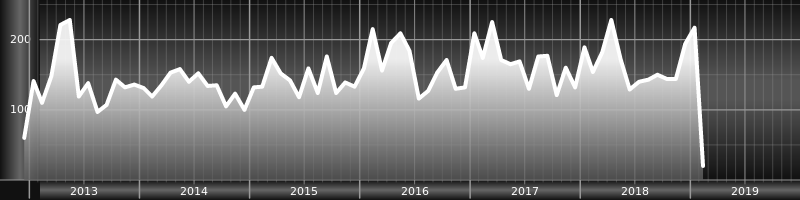
\includegraphics[width=\linewidth]{CTAN}}%
   [Short caption B]%
   {A Caption B of a ``fullpage'' sub object.}%  subcaption
   {}%
  +{}{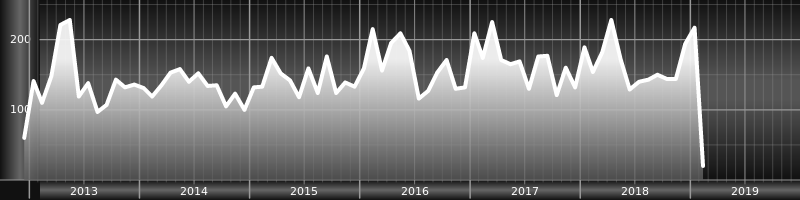
\includegraphics[width=\linewidth]{CTAN}}%
   {A Caption C of a ``fullpage'' object, which follows on the left or right column.}%
   {sub:demo1}
  +{}{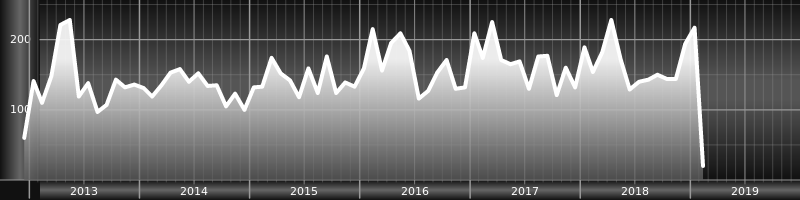
\includegraphics[width=\linewidth]{CTAN}}%
   {A Caption D of a ``fullpage'' object}%
   {sub:demo2}
  +{}{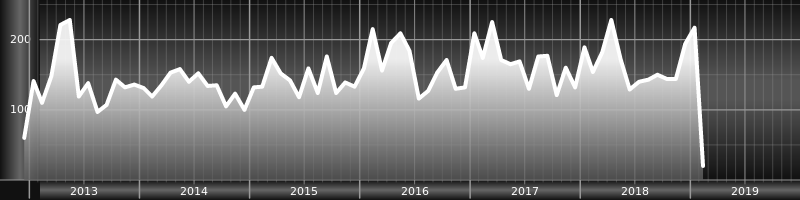
\includegraphics[width=\linewidth]{CTAN}}%
   {A Caption E of a ``fullpage'' object}%
   {sub:demo3}
\end{lstlisting}

\Float[subfloat]
\captionsetup[sub]{singlelinecheck}
\hvFloat[fullpage,capPos=l,objectFrame,subFloat]%
  +{figure}{}[Short main caption of the objects]%   main short lsi entry
   {The main  caption of a ``fullpage'' object, which follows on the left or
        right column. This can be an even or odd page. And some more text whch has no
        real meaning because it fills only the space for a long caption.}%  main caption
   {sub:demo0}%
  +{}{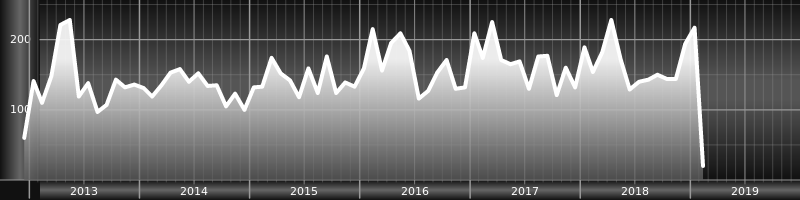
\includegraphics[width=\linewidth]{CTAN}}%
   [Short caption B]%
   {A Caption B of a ``fullpage'' sub object.}%  subcaption
   {}%
  +{}{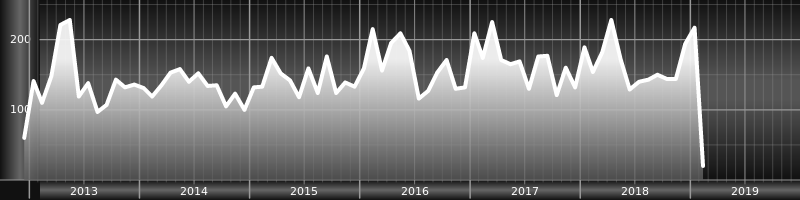
\includegraphics[width=\linewidth]{CTAN}}%
   {A Caption C of a ``fullpage'' object, which follows on the left or right column.}%
   {sub:demo1}
  +{}{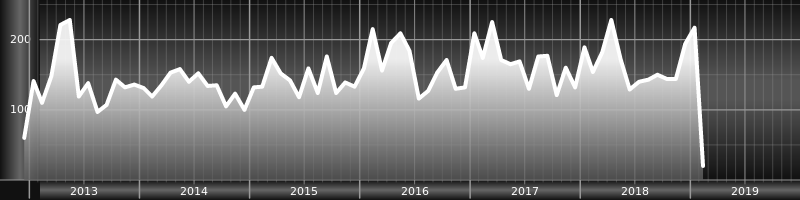
\includegraphics[width=\linewidth]{CTAN}}%
   {A Caption D of a ``fullpage'' object}%
   {sub:demo2}
  +{}{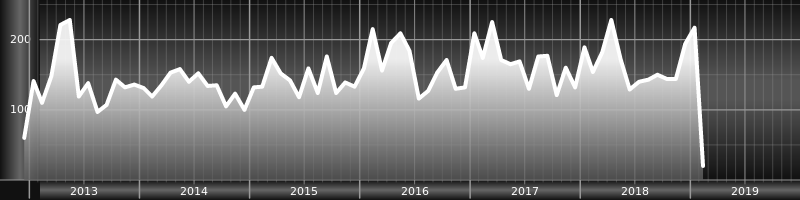
\includegraphics[width=\linewidth]{CTAN}}%
   {A Caption E of a ``fullpage'' object}%
   {sub:demo3}



\blinddocument


\begin{lstlisting}
\captionsetup[sub]{singlelinecheck}
\hvFloat[fullpage,capPos=l,objectFrame,subFloat]%
  +{figure}{}[Short main caption of the objects]%   main short lsi entry
   {The main  caption of a ``fullpage'' object, which follows on the left or
        right column. This can be an even or odd page. And some more text whch has no
        real meaning because it fills only the space for a long caption.}%  main caption
   {sub:demo4}%
  +{}{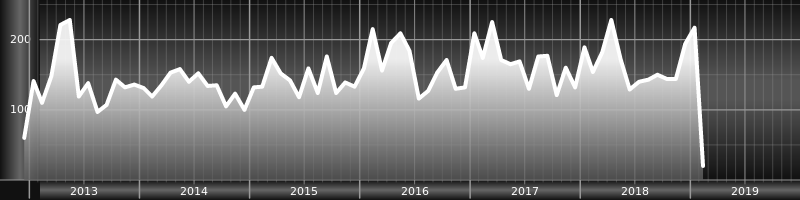
\includegraphics[width=\linewidth]{CTAN}}%
   [Short caption B]%
   {A Caption B of a ``fullpage'' sub object.}%  subcaption
   {}%
  +{}{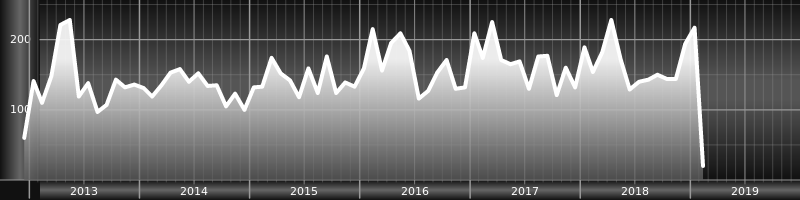
\includegraphics[width=\linewidth]{CTAN}}%
   {A Caption C of a ``fullpage'' object, which follows on the left or right column.}%
   {sub:demo5}
  +{}{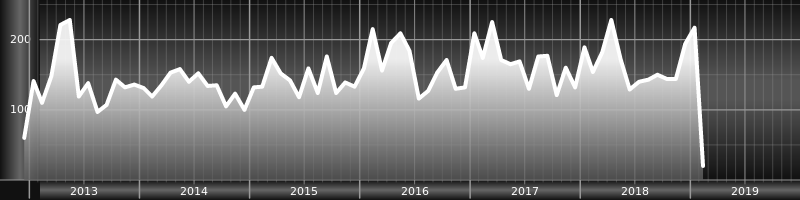
\includegraphics[width=\linewidth]{CTAN}}%
   {A Caption D of a ``fullpage'' object}%
   {sub:demo2}
  +{}{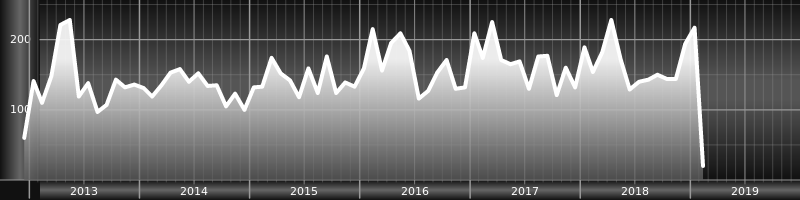
\includegraphics[width=\linewidth]{CTAN}}%
   {A Caption E of a ``fullpage'' object}%
   {sub:demo6}
\end{lstlisting}

\Float[subfloat]
\captionsetup[sub]{singlelinecheck}
\hvFloat[fullpage,capPos=l,objectFrame,subFloat]%
  +{figure}{}[Short main caption of the objects]%   main short lsi entry
   {The main  caption of a ``fullpage'' object, which follows on the left or
        right column. This can be an even or odd page. And some more text whch has no
        real meaning because it fills only the space for a long caption.}%  main caption
   {sub:demo4}%
  +{}{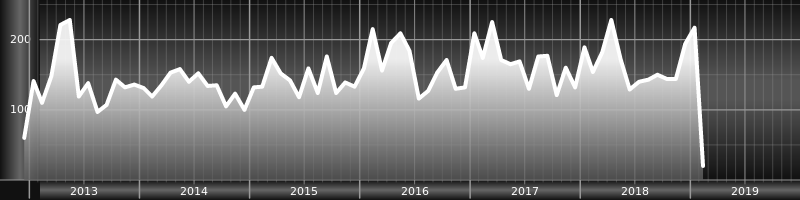
\includegraphics[width=\linewidth]{CTAN}}%
   [Short caption B]%
   {A Caption B of a ``fullpage'' sub object.}%  subcaption
   {}%
  +{}{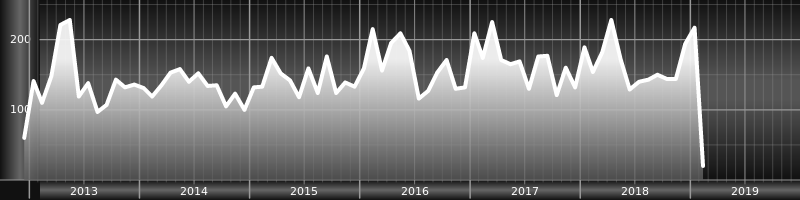
\includegraphics[width=\linewidth]{CTAN}}%
   {A Caption C of a ``fullpage'' object, which follows on the left or right column.}%
   {sub:demo5}
  +{}{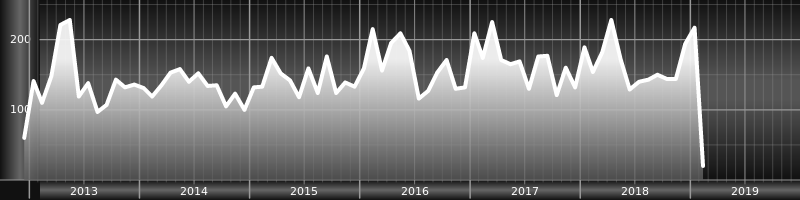
\includegraphics[width=\linewidth]{CTAN}}%
   {A Caption D of a ``fullpage'' object}%
   {sub:demo7}
  +{}{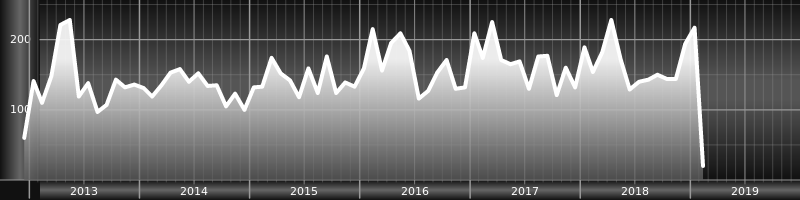
\includegraphics[width=\linewidth]{CTAN}}%
   {A Caption E of a ``fullpage'' object}%
   {sub:demo6}



\blinddocument

\Blindtext

\blindtext


\end{document}